
Za usporedbu, odabranu su sljedeća tri modela:

\begin{itemize}
    \item WGAN - model Pix2pix uz Wasserstein GAN\cite{pix2pixwgan}
    \item ParGN - paralelni model temeljen na GAN-ovima\cite{kumar2022paracolorizer} 
    \item InstColor - Instance-aware Image Colorization\cite{Su_2020_CVPR}
\end{itemize}

Njihove mjere dobrote IS i FID usporedno su prikazane u tablici \ref{table:usporedne_mjere}. Nažalost, mjera IS nije izračunata u modelima ParGN\cite{kumar2022paracolorizer} i InstColor\cite{Su_2020_CVPR}. Dodatno, mjera FID prikazana je stupčastim dijagramom \ref{fig:fid_comp}, a mjera IS prikazana je za dva modela kao graf normalnih distribucija \ref{fig:is_comp}.

\begin{table}[H]
    \centering
    \caption{Usporedba mjera dobrote modela}
    \label{table:usporedne_mjere}
    \begin{tabular}{ |c|c|c|c|c|c| }
        \hline
         & \multicolumn{2}{|c|}{stvarne slike} & \multicolumn{2}{|c|}{obojene slike} &  \\
        \hline
        Model & IS $\mu$ & IS $\sigma$ & IS $\mu$ & IS $\sigma$ & FID \\
        \hline
        \hline
        cGAN & \textbf{5.2293} & \textbf{1.2776} & \textbf{5.1197} & \textbf{1.2776} & 8.5348 \\
        \hline
        WGAN\cite{pix2pixwgan} & 4.1913 & 1.7591 & 4.2828 & 1.9007 & 36.9385 \\
        \hline
        ParGN\cite{kumar2022paracolorizer} & - & - & - & - & 16.8273 \\
        \hline
        InstColor\cite{Su_2020_CVPR} & - & - & - & - & \textbf{7.36} \\
        \hline
    \end{tabular}
\end{table}


\begin{figure}
    \centering
    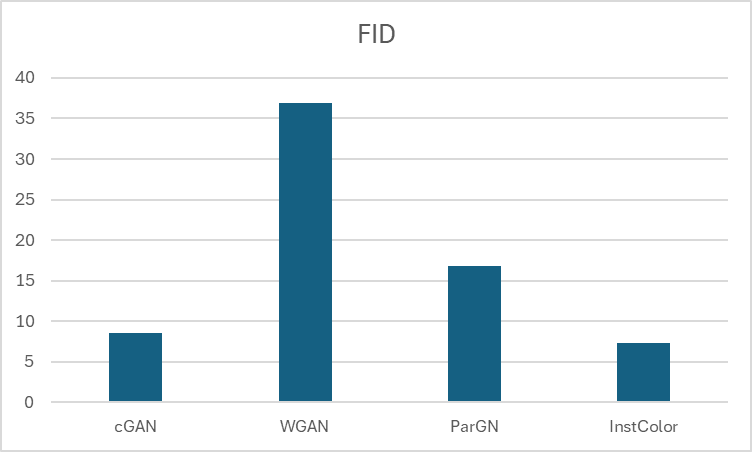
\includegraphics[width=0.75\linewidth]{imgs/fid_corrected.png}
    \caption{Stupčasti dijagram FID-ova modela}
    \label{fig:fid_comp}
\end{figure}


Kao što možemo vidjeti na prikazanom stupčastom dijagramu \ref{fig:fid_comp}, naš model (cGAN) ima značajno bolji iznos mjere FID od modela WGAN\cite{pix2pixwgan} i ParGN\cite{kumar2022paracolorizer}, ali ne toliko dobar kao model InstColor\cite{Su_2020_CVPR}. To bi mogao biti rezultat ekstrakcije značajki objekata iz slika koje provodi model InstColor\cite{Su_2020_CVPR}.

\begin{figure}[H]
    \centering
    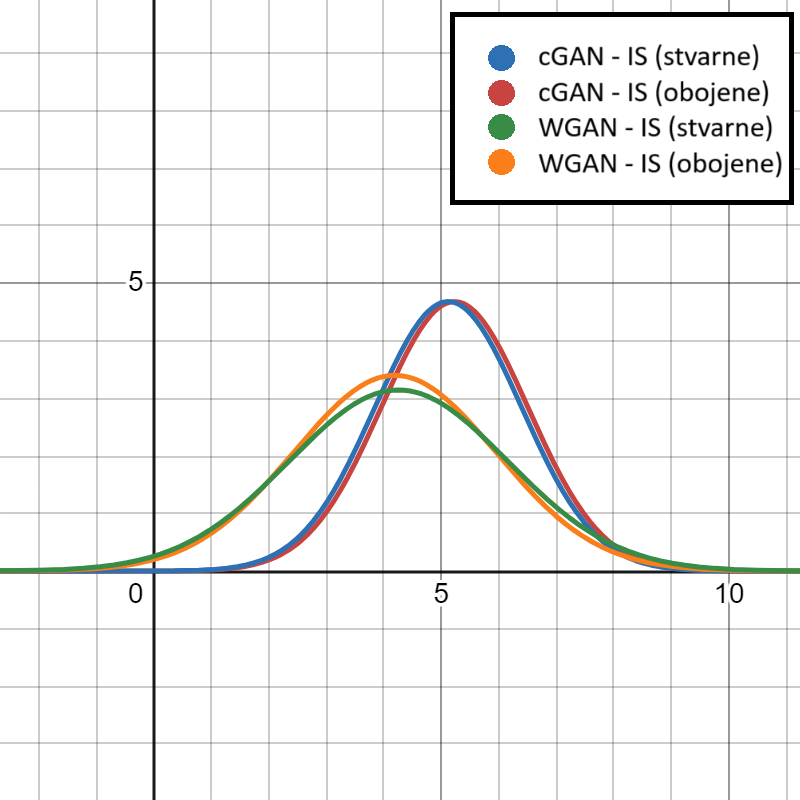
\includegraphics[width=0.75\linewidth]{imgs/is_comp.png}
    \caption{Graf IS-ova modela}
    \label{fig:is_comp}
\end{figure}

Kao što možemo vidjeti na grafu \ref{fig:is_comp}, naš model (cGAN) ima veći iznos mjere IS od modela WGAN\cite{pix2pixwgan}, uz manju standardnu devijaciju. Prema tome, naše obojene slike sličnije su stvarnim slikama u usporedbi s obojenim slikama dobivenim modelom WGAN\cite{pix2pixwgan}. Model WGAN\cite{pix2pixwgan} ima manju razliku središnje vrijednosti između stvarnih i obojenih slika iznosa $0.0915$, dok model cGAN ima razliku iznosa $0.1096$. Ipak, može se reći da cGAN ima bolji iznos mjere IS zbog znatno manje standardne devijacije, kao i općenito većeg iznosa.